%%%%%%%%%%%%%%%%%%%%%%%%%%%%%%%%%%%%%%%%%%%%%%%%%%%%%%%%%%%%%%%%%%%%%%%%%%%%%%%%
%%                           ONDER DE LOEP ARTIKEL                            %%
%%%%%%%%%%%%%%%%%%%%%%%%%%%%%%%%%%%%%%%%%%%%%%%%%%%%%%%%%%%%%%%%%%%%%%%%%%%%%%%%

\artikelfoto{Basisgeletterdheid wiskunde in de eerste graad A- en B-stroom}{}{Filip Moons}{img/ikea.jpg}

\startcontents[inhoudloep]	% om inhoud voor het loep artikel te beginnen

\begin{multicols}{2}
	
	\inhoudstafelloep			% om inhoudstafel voor het loep artikel te tonen
	
	%% Gebruik \section{titel} en \subsection{titel} om genummerde tussentitels te maken
\section{Inleiding}
De hervorming van het secundair onderwijs in de eerste graad bracht, naast nieuwe eindtermen voor de A- en de B-stroom, ook eindtermen basisgeletterdheid voor wiskunde, Nederlands, digitale competenties en financiële geletterdheid met zich mee. We spreken dus van `Basisgeletterdheid wiskunde' en helaas niet over gecijferdheid, omdat ook de andere kennisgebieden voorzien werden van een pakketje eindtermen basisgeletterdheid. Basisgeletterdheid omvat een aantal essentiële eindtermen (27 stuks, waarvan 7 die onder wiskunde vallen) die je nodig hebt om als geletterde en gecijferde burger aan de maatschappij te kunnen participeren. Daarom moeten ze op individueel niveau bereikt worden. Dat is anders dan de reguliere eindtermen die op `populatieniveau' moeten worden bereikt. Dit wil zeggen dat een zo groot mogelijk aantal leerlingen deze eindtermen moet behalen. Als vuistregel hanteert men meestal dat `70\% van de leerlingen de eindtermen moeten behalen', al blijft dit een theoretische doelstelling.

In deze loep verdiepen we ons in de wiskundige inhoud van deze eindtermen basisgeletterdheid. We reiken haalbare ideeën aan om zinvol en met de nodige diepgang met deze doelen in de klas om te gaan. Wie de geest van deze doelen leest, merkt dat het veeleer over `gecijferdheid' gaat dan over pure wiskunde. We starten daarom met een omschrijving van gecijferdheid. Vervolgens kijken we naar een aantal evoluties die de invoering van de eindtermen basisgeletterdheid wiskunde verklaren. Daarna onderzoeken we hoe die eindtermen exact zijn opgesteld en op welke manier ze geïntegreerd kunnen worden in de reguliere (wiskunde)lessen. We sluiten af met een hoofdstuk over het evalueren van de basisgeletterdheid en een korte blik op het masterproefonderzoek dat Enya Vermeyen en Britt Lenaerts over dit onderwerp uitvoerden in het kader van de educatieve master wiskunde aan de UAntwerpen. Doorheen deze loep vind je enkele voorbeelden uit het B+ project, een prioritaire nascholing voor wiskunde in de B-stroom gesubsidieerd door de Vlaamse overheid en georganiseerd door het Provinciaal Onderwijs Vlaanderen, PXL Hogeschool en de Universiteit Antwerpen.

In de loep vind je op verschillende plekken, eerder willekeurig verspreid, een aantal lesideeën. Dit zijn illustraties van mogelijke lesactiviteiten die je kan ontwerpen of tools die je kan gebruiken om aan de basisgeletterdheid wiskunde te werken. 

\section{Wat is gecijferdheid?}
	\begin{citaat}[Prof. Frederik van der Blij, 1995] % auteur is optioneel argument
		Ik denk dat je gecijferd bent als je mensen die je willen
bedriegen kunt ontmaskeren.
	\end{citaat}
\subsection{Geschiedenis}
Om zicht te krijgen op  het begrip gecijferdheid katapulteren we onszelf terug naar het jaar des Heren 1602. Op dat moment wordt de `vereenigde Oostindische Compagnie' bij onze Noorderburen opgericht (Balk et al., 2007), wat in de geschiedenis gezien wordt als de allereerste multinational. De opkomst van de internationale handel doet al in de vroege middeleeuwen de behoefte ontstaan aan geschreven documenten en vooral boekhoudingen. Het is via deze internationale tendens dat op school rekenen als apart vak ingang vindt. 

Een traditionele rekenles bestond in die tijd uit de schoolmeester die instrumenteel, stap-voor-stap een rekenprocedure aan de klas uitlegde. Vervolgens oefenden de leerlingen deze procedure in door een indrukwekkende hoeveelheid `kale' oefeningen te maken. De `leerlingen', vooral afkomstig uit de adel en de rijke burgerij, leerden zo snel en zo goed mogelijk `rekenen'. Contexten of realistische opgaven, die vandaag een duidelijke plaats in het onderwijs hebben, kregen weinig of geen aandacht. De vertaalslag moesten de leerlingen zelf maken. 

Wanneer je een schoolboek wiskunde van het basisonderwijs van bijvoorbeeld 1950 openslaat, zal je zal merken dat het `mechanistisch rekenen' met het accent op dril veel aandacht krijgt. Cijferen en het aanleren van procedures zijn prominent aanwezig. Soms werden wel vraagstukken opgelost, maar vooral de nadruk op dril was frappant. 

Pas in de tweede helft van de 20ste eeuw verandert het denken hierover, met in de Lage Landen, bekende namen als Hans Freudenthal (1967). Hij raakte steeds meer overtuigd van de rol van wiskundeonderwijs als `dienstbaar vakgebied' en de noodzaak om kinderen te leren deze wiskunde te herkennen en te kunnen gebruiken in alle mogelijke situaties. Het duurde nog tot eind jaren '80 voordat in Vlaanderen deze visie meer ingang vond. 

Twintig jaar later, we schrijven 1988, laat de Amerikaanse wiskundige John Allen Paulos zijn boek `Innumeracy, mathematical illiteracy and its consequences' op de wereld los. In het boek betoogt Paulos dat ongecijferdheid een groot probleem vormt voor een steeds groter aantal mensen, bij wie het verder niet aan gezond verstand ontbreekt. 

Zo concluderen de meeste mensen uit het weerbericht `zaterdag 50\% kans op regen en zondag 50\% kans op regen', dat er dit weekend 100\% kans op regen te verwachten is. Het antwoord is in werkelijkheid onbekend, aangezien het regenen op zondag beïnvloed wordt door het weer op zaterdag. Wie zich onafhankelijk van deze natuurwetten opstelt, komt overigens nog steeds niet bij 100$\%$, maar bij 75$\%$ kans op regen. 

In een ander voorbeeld over de loterij laat Paulos zien dat men gemiddeld genomen altijd beduidend veel meer geld verliest aan het kopen van loten dan de winst die men mag verwachten. Hij beschouwt het als volstrekt irrationeel gedrag dat miljoenen mensen wekelijks deelnemen aan kras- en lottospelen allerhande. Een kanttekening hierbij is natuurlijk wel dat de kans om millionair te worden groter is als je lotjes koopt dan als je er geen koopt. 

\end{multicols}
 \afbeelding[14 cm]{img/kans.jpg}{}{}
 \begin{multicols}{2}


Het boek groeit al gauw uit tot een internationale bestseller. Het verandert, samen met gelijkaardige tendensen, vrij snel het denken over de rol van wiskunde in het dagelijks leven en zet het probleem van (on)gecijferdheid op de kaart.

Waar Paulos sterk de nadruk legt op kansrekening, doen anderen dat veel minder. Zo omschrijft Kees Hoogland in 1997 gecijferdheid als ‘IKEA-wiskunde’. Immers bij IKEA:
\begin{itemize}
    \item vind je je weg op basis van een grondplan, 
    \item moet je vooraf je kamer opmeten,
    \item vergelijk je met de maten in de winkel, 
    \item zoek je informatie over producten en vergelijk je die voor verschillende producten,
    \item steek je op basis van een bouwplan de aangekochte waren in elkaar,
    \item en kun je, ten slotte, op krediet kopen met de IKEA-kaart.
\end{itemize}

Kortom, allerlei vaardigheden in verband met gecijferdheid vind je bij de Zweedse meubelgigant. 

Als in 2000 de Organisatie voor Economische Samenwerking en Ontwikkeling (OESO) voor het eerst start met het grootschalige internationaal vergelijkend onderzoek PISA (Programme for International Student Assessment), waarbij leerlingen in verschillende landen op de leeftijd van 15 jaar vergeleken worden op gebied van taal, wiskunde en wetenschappen, is iedereen zich bewust van het belang van gecijferdheid. In tegenstelling tot wat velen denken, meet PISA niet rechtstreeks de kennis van de wiskunde-inhouden van het middelbaar onderwijs, maar eerder een andere notie van `wiskundige geletterdheid’:
\begin{citaat}[Wiskundige geletterdheid volgens PISA] 
    Wiskundige geletterdheid is de vaardigheid van een individu om de rol van wiskunde in de wereld te identificeren en te begrijpen, om gefundeerde afwegingen te maken en om wiskunde te gebruiken en ermee te interageren zodat het een leven mogelijk maakt als een constructieve, betrokken en reflectieve burger in deze maatschappij.
\end{citaat}


\end{multicols}
 \afbeelding[12 cm]{img/ikea wiskunde.jpg}{}{}
 \begin{multicols}{2}

\subsection{Voorbeelden}
Om niet in abstracte begrippen te blijven hangen, geven we een aantal voorbeelden die het belang weergeven van gecijferdheid in verschillende domeinen.\\


\noindent\textbf{Voorbeeld 1: Het spotten van onmogelijke of verkeerde berekeningen}\\

\afbeelding{img/colruyt.png}{Zeer goedkope champagne bij Colruyt}{champagne}

Een zeer bekend voorbeeld van gecijferdheid is het spotten van promoties die te mooi zijn om waar te zijn. Wat dacht je van een fles champagne van Laurent-Perrier aan 2 euro in de Colruyt (\autoref{champagne}) of tuinlampionnen die 60$\%$ dalen in prijs bij Hema i.p.v. de gemarkeerde $20\%$ (\autoref{lampion})? De link met gecijferdheid is evident: een gecijferd persoon heeft normaliter genoeg inschattingsvermogen om meteen door te hebben dat er iets niet in de haak is met deze promoties, zonder dat de promotie moet nagerekend worden.

\afbeelding{img/tuinlampion.png}{Opvallende promotie bij Hema}{lampion}

Een aardig weetje: een overduidelijk foute prijs in een advertentie verplicht de handelaar volgens de wet niet om het product aan die lage prijs te verkopen. De kaarten liggen anders als die prijs ook in de winkel aangegeven is:   dan spreken we van een effectief aanbod, en dan mag men aan de kassa niet zeggen dat het product eigenlijk duurder is.

%\vspace{0.5 cm}

\noindent \textbf{Voorbeeld 2: Misleidende grafieken en tabellen ontmaskeren}\\
Eind 2020 plaatste de senaatvoorzitter Stephanie D'Hose de grafiek in \autoref{dhose} op haar Facebookpagina.

\afbeelding{img/dhose.jpg}{Een budget van 13 miljoen euro per jaar voor de Senaat?}{dhose}



De Senaat, sinds enkele staatshervormingen een enigszins stoffige instelling in het Belgisch politiek bestel, houdt slechts een budget over van $\euro39,6$ miljoen in 2021 ten opzicht van $\euro 80$ miljoen in 2013. Dat is een fikse besparing, maar de grafiek suggereert een nog veel grotere besparing: als je echt de staven in verhouding zou opmeten, zou de Senaat het moeten rooien met 13 miljoen euro in 2021 en de halvering van het budget zou volgens de grafiek al een feit zijn in 2014. Een erg misleidende grafiek dus. 

Ook politieke partijen die omhoog gaan in peilingen, bedienen zich op sociale media traditioneel van grafieken die een veel spectaculairdere stijging suggereren. Zelfs een dusdanige misleiding met een verdubbeling in stemmenaantal -- wat in de Belgische politiek bijna nooit voorkomt -- is vaak niet uitgesloten.

\textbf{Voorbeeld 3: Proportioneel redeneren}\\
Een ander aspect is proportioneel denken of denken in verhoudingen. 

Eén van de meest voor de hand liggende voorbeelden is een recept, zoals in \autoref{libelle}, waar de ingrediëntenlijst  voor 6 personen wordt gegeven. 

\afbeelding{img/libelle.jpg}{Hoeveel ingrediënten nodig voor vier personen?}{libelle}

Als je slechts 4 gezinsleden hebt, moet je in staat zijn om in te schatten wat je minder hoeft te kopen en je toch genoeg ingrediënten voor je hele gezin meeneemt. 

Dit voorbeeld illustreert meteen het verschil tussen wiskunde en gecijferdheid. Uiteraard kunnen we dit met verhoudingen, `de regel van drie' of zelfs met breuken, éxact uitrekenen hoe de ingrediëntenlijst er voor vier personen uitziet, maar in realiteit zullen we dit zelden doen. 

Gewoonlijk maken we een snelle inschatting waarbij we enerzijds schatten wat voldoende is voor 4 personen, maar anderzijds ook rekening houden met het aanbod in de supermarkt. De supermarkt biedt waarschijnlijk een doos kipfiletblokjes van 420 g of 200 g aan, terwijl je wiskundig gezien 266,6 g nodig hebt. Voor vier personen heb je voldoende aan een half zakje woksaus maar dat ligt uiteraard niet in de winkel. Hoewel je de wiskundige inschatting nodig hebt om een juiste beslissing te nemen, kan de samenstelling van het gerecht hierdoor toch lichtjes afwijken.

Een recept is een goed gekend voorbeeld waarbij je proportioneel denkt. Het maken van een prijsvergelijking (met verschillende offertes) of een keuze tussen een iPhone en iPhone Pro (waar de grootte van het scherm verschillend is),... spreken datzelfde proportioneel denken aan. \\

\noindent \textbf{Voorbeeld 4: Inschattingen maken}\\
\noindent Inschattingen kunnen maken is een ander belangrijk onderdeel van gecijferdheid. We geven enkele voorbeelden om te verduidelijken hoe mensen in het dagelijkse leven - soms onbewust - inschattingen maken op basis van een aantal elementen die meespelen. 

In \autoref{sintniklaas} vind je een advertentie voor de huur van een appartement. De prijs, $\euro 900$ per maand, is een vrij hoge prijs voor een appartement in Sint-Niklaas. Onbewust vergelijk je al met appartementen waarvan je de prijs al kent. Een ander element dat meespeelt in het bepalen van een prijs is de grootte van het appartement. Met 173m$^2$ krijg je er effectief een heel grote leefruimte voor in de plaats. Ook hier zet je weer cijferkennis in om een oordeel te vormen. En ook de locatie speelt mee: de Statiestraat - wisten enkele Waaslanders te vertellen - is nu eenmaal thé place to be in Sint-Niklaas. Als je rekening houdt met al deze elementen valt de huurprijs te rechtvaardigen. 
\afbeelding{img/sintniklaas.jpg}{Aanvaardbare prijs?}{sintniklaas}

Een ander voorbeeld vinden we bij ‘abonnementen voor diensten'. In veel steden komt de Swapfiets in zwang (zie \autoref{swapfiets}). Voor een kleine $\euro 20$ per maand kun je een persoonlijke fiets huren. Daar zijn een aantal voordelen aan. Als er iets met de fiets mis is, kun je die meteen ruilen voor een nieuwe. In het servicepunt kun je gratis je banden laten oppompen. 

Welke afwegingen maak je best vooraf vooraleer je zo'n abonnement aangaat? Interessante vragen daarbij zijn: vanaf wanneer is zo'n abonnement te verkiezen boven het kopen van een (tweedehands)fiets? Na hoeveel maanden heb je evenveel geld gespendeerd aan je abonnement als je kwijt bent voor de aanschaf van een nieuwe fiets? Bovendien is aandacht voor de kleine lettertjes belangrijk: wiens fiets gestolen wordt en het sleuteltje nog heeft, betaalt eenmalig $\euro 60$; wie ook het sleuteltje kwijtspeelt, betaalt eenmalig $\euro 450$. 

Daarnaast zijn er belangrijke randvoorwaarden die meewegen in de beslissing om voor een Swapfiets te kiezen: ben je vergeetachtig en durf je weleens je fiets vergeten op slot te doen? Dan verdient een eigen (tweedehands)fiets zeker de voorkeur. Ben je bedachtzaam en heb je maar voor beperkte tijd een fiets nodig? Dan is een Swapfiets een optie. 

Twintig euro lijkt overigens weinig als je die prijs vergelijkt met de dagprijs voor het huren van een fiets op een toeristische bestemming. Als toerist betaal je ongeveer 20 euro voor het het huren van een fiets in het Italiaanse stadje Polignano, dat lijkt in verhouding tot de Swapfiets, dan weer onredelijk veel. Al blijft het daar kiezen tussen die twintig euro of niet fietsen in Italië...  

Dit soort voor- en nadelen goed kunnen afwegen valt onder gecijferdheid.

\afbeelding{img/swapfiets.jpg}{Interessante deal of niet?}{swapfiets}

Meer alledaagse inschattingen - die voor gecijferde personen erg voor de hand liggen - vallen ook onder deze vaardigheid. Bijvoorbeeld kunnen inschatten hoe vroeg je moet opstaan om op tijd op school te geraken, een reistijd kunnen inschatten, kunnen sparen voor een grotere aankoop, het juiste geld sparen voor een gsm-abonnement, kunnen inschatten of de vrije ruimte tussen twee auto's voldoende is om er tussen te parkeren... zijn allemaal vaardigheden die onder gecijferdheid vallen.

Mensen in socio-economisch zwakkere situaties zijn vaak minder gecijferd dan medeburgers die welgestelder zijn. De theorie van Eldar Shafir van de Univeristeit van Princeton (Bregman, 2013) stelt dat dit proces in twee richtingen werkt: mensen in armoede ervaren vaak een constante, langdurige stress die een negatief effect heeft op de mogelijkheid om een goede keuze te maken. Onderzoek toonde ook aan dat wanneer mensen in ernstige financiële moeilijkheden geraken, het IQ gemiddeld met 13 punten afneemt. Dit is vergelijkbaar met een nacht niet slapen. Men heeft minder `bandbreedte' en maakt meer korte termijn besluiten. Mensen hebben `teveel aan hun hoofd’. De acute geldproblemen nemen je in beslag, daardoor is er minder aandacht voor de lange termijn en is men alleen bezig met zijn of haar primaire behoeften.


\textbf{Andere voorbeelden}\\
Andere alledaagse situaties waarin een kwantitatieve blik op de wereld een grote rol speelt en waarvoor gecijferdheid dus belangrijk is:
\begin{itemize}
    \item Je oriënteren met een kaart.
    \item In een vreemde stad de metroroute uitstippelen met een metroplan.
    \item Aan een bushalte de uurregeling aflezen.
    \item Van een factuur inschatten of die kan kloppen of niet.
    \item Zich bewust zijn dat bij het lenen van geld, een veel groter bedrag moet terugbetaald worden dan enkel het geleende bedrag.
    \item Bij het deelnemen aan kansspelen of sportweddenschappen beseffen dat de winstverwachting altijd negatief is.
    \item ...
\end{itemize}

\subsection{Verschil tussen wiskunde en gecijferdheid}
Uit voorgaande voorbeelden blijkt dat gecijferdheid toch wat anders dan het vak wiskunde is. Gecijferdheid heeft altijd te maken met heel concrete situaties uit het dagelijkse leven. Het gaat over het interpreteren van numeriekee of ruimtelijk/meetkundige informatie, numerieke informatie naar waarde kunnen schatten, waar nodig is er kritisch over zijn en vervolgens een mening of besluit te vormen. 

Het vak wiskunde zoals we dat kennen draagt ongetwijfeld bij tot gecijferdheid, maar heeft ook andere doelstellingen en is abstracter van aard. Tijdens wiskundelessen werken we geregeld zonder contexten, ligt er ook nadruk op technieken of formele notaties. De oefeningen hebben vaak een juist antwoord, waarbij een mening of besluit vormen vaak niet het doel is. Dit verschilt natuurlijk van les tot les: een modelleeropdracht sluit meer aan bij op opbouwen van gecijferdheid dan een les pure algebra. 

Verderop zal blijken dat dit verschil zich uit in andere accenten tussen de reguliere eindtermen en de eindtermen basisgeletterdheid wiskunde. We mogen er als wiskundeleraars niet van uitgaan dat gecijferdheid een automatisch bijproduct is van onze wiskundelessen dat sowieso gehaald wordt als het vak wiskunde gehaald wordt.


\section{Basisgeletterdheid invoeren}
\subsection*{Stijgende groep laaggecijferden}

De invoering van de eindtermen basisgeletterdheid in de eerste graad werd ingeschreven in het `Strategisch Plan Geletterdheid' van de Vlaamse Overheid. Dit plan wil de geletterdheid bij jongeren, werkzoekenden, werkenden en bij mensen in armoede in Vlaanderen verhogen. 

De aanleiding is rechtstreeks terug te brengen op het snel stijgende groep laagpresteerders in Vlaanderen in PISA-testen. PISA is een grootschalig internationaal vergelijkend onderzoek dat wordt uitgevoerd in de OESO. De laatste afname was in 2018. PISA test taal, wiskundige en wetenschappelijke vaardigheden. 

In tegenstelling tot wat weleens gedacht wordt, peilt PISA naar algemene vaardigheden die verwacht kunnen worden op de leeftijd van 15 jaar. Het test dus niet rechtstreeks het wiskundecurriculum zoals dat bij peilingsproeven of TIMMS (Trends in International Mathematics and Science Study) wel het geval is. 

De TIMSS-toetsen zijn vierjaarlijkse toetsen (sinds 1995) wiskunde en wetenschappen die bij leerlingen uit het 4de leerjaar lager onderwijs (internationaal aangeduid als grade 4) en bij leerlingen uit het 2de jaar van de 1ste graad secundair onderwijs (grade 8) worden afgenomen. TIMSS sluit, in tegenstelling tot PISA, veel nauwer aan bij de wiskunde die in de klas wordt behandeld. 

Voor PISA participeert voor Vlaanderen een steekproef van 8000 15-jarigen. Daarbij is enkel de leeftijd een deelnamecriterium, niet in welk jaar de leerling zit. Men test 15-jarigen omdat in veel landen het leerplichtonderwijs stopt op 16 jaar en het dus een ideaal referentiepunt is om onderwijssystemen met elkaar te vergelijken. 

PISA heeft verschillende vaardigheidsniveaus waarbij bij elke stijging van het niveau meer abstracte vaardigheden worden verwacht. Niveau 1 gaat over het kunnen beantwoorden van eenduidige vragen in goed gekende contexten, waarbij de corresponderende bewerking voor de hand ligt. Niveau 2 komt overeen met het beheersen van een zeer rudimentair basisarsenaal van rekenvaardigheden met gehele getallen zonder veel achterliggend denkwerk (zie de onderstaande kader voor een diepgaandere uitleg). PISA beschouwt leerlingen als laaggecijferd als ze onder referentieniveau 2 scoren. Wie dit niveau niet haalt en dus op niveau 1 of lager presteert, is volgens PISA laaggecijferd.   

\begin{kader}{PISA Mathematics Framework}{Niveau 2}

Leerlingen op niveau 2 kunnen situaties interpreteren en herkennen in
contexten waarin alle informatie direct af te leiden is. Ze kunnen
relevante informatie uit een eenvoudige bron halen en kunnen een
enkelvoudige representatie gebruiken. Leerlingen kunnen op dit niveau
elementaire algoritmes, formules, procedures of conventies gebruiken om
opgaven met gehele getallen op te lossen. Ze zijn in staat om resultaten letterlijk te interpreteren. 
	\end{kader}
	

In de laatste PISA-meting van 2018, presteerde 17,3$\%$ van de Vlaamse leerlingen onder dat referentieniveau 2. In de \autoref{tab:pisa} zie je onder niveau 2: $11,3\% + 6\% = 17,3\%$. Eén Vlaamse leerling op zes beschikt op 15-jarige leeftijd niet over een basis aan wiskundige vaardigheden om vlot mee te draaien in deze maatschappij. 
\begin{tabel}
	\begin{tabular}{crr}
		\hlinethick
	\tableheader{Niveau}       & 	\tableheader{OESO-gemiddelde} & 	\tableheader{Vlaanderen}    \\
	\hlinethick
6            & 2,4\% (0,1)     & 4,4\% (0,53)  \\
5            & 8,5\% (0,1)     & 14,4\% (0,80) \\
4            & 18,5\% (0,1)    & 23,6\% (0,95) \\
3            & 24,4\% (0,1)    & 23,1\% (0,97) \\
		\hlinethick

2            & 22,2\% (0,1)    & 17,2\% (0,73) \\
	\hlinethick

1            & 14,8\% (0,1)    & 11,3\% (0,83) \\
\textless{}1 & 9,1\% (0,1)     & 6,0\% (0,85) 
\end{tabular}
	\caption{Percentage leerlingen per wiskundig vaardigheidsniveau gemiddeld over de OESO-landen en in Vlaanderen. De standaardfout staat tussen haakjes.} \label{tab:pisa}
\end{tabel}
Dat die cijfers zorgen moeten baren, blijkt onder meer uit het feit dat Vlaanderen een significante stijging kent van het aandeel laaggecijferden. In 2003 was die groep nog beperkt tot 11,4$\%$ (zie \autoref{tab:pisa2}). 

Bovendien staat deze stijging in Vlaanderen in contrast met het stabiel blijven van deze groep over alle OESO-landen heen. Meer dan de helft (58$\%$) van de laaggecijferde leerlingen bevinden zich in het (deeltijds) beroepsonderwijs. Toch mag noch het tso, noch het aso op zijn lauweren rusten. Maar liefst 4,8$\%$ van de laaggecijferde leerlingen volgde in 2018 les in het aso, een verzesvoudiging (!) ten opzichte van 2003. Daarnaast huist 18,5$\%$ van de laaggecijferden in het tso. De overige percentages situeren zich in de eerste graad (leerlingen die niet op leeftijd zitten) of het kso. 

Eenvoudige verklaringen zoals het feit dat migratie een rol zou spelen in deze stijgende cijfers, blijken niet afdoende. Niet alleen is het aandeel van migranten over de meetmomenten heen onveranderd gebleven, andere landen met gelijkaardige migratiepatronen, slagen er toch beter in om hun groep laaggecijferden klein of op z’n minst stabiel te houden.

\end{multicols}
\begin{tabel}
	\begin{tabular}{lrrrrrr}
	\hlinethick
 \tableheader{}& \multicolumn{1}{c}{\tableheader{PISA2003}} & \multicolumn{1}{c}{\tableheader{PISA2012}} & \multicolumn{1}{c}{\tableheader{PISA2018}} \\
  \hlinethick
OESO & 21,6\% (0,2)  & 22,2\% (0,2)  & 22,1\% (0,2) \\
Vlaanderen      & \textbf{11,4\% (0,6)}  & 15,4\% (1,1) & 17,3\% (1,3) 
\end{tabular}
	\caption{Percentage laagpresteerders oor wiskunde. Vergelijk PISA20003, PISA2012 en
PISA2018. Vetgedrukte getallen wijzen op significante verschillen t.o.v. 2018} \label{tab:pisa2}
\end{tabel}
\begin{multicols}{2}

 Verder toont PIAAC (Programme for the International Assessment of Adult Competencies), vergelijkbaar met PISA maar dan voor volwassenen, een gelijkaardig beeld waarbij 1 op 7 volwassen in Vlaanderen laaggeletterd (breder dan wiskunde alleen) is, met een gigantische digitale kloof tussen de jongere en oudere generaties. De jongere generatie is veel digitaler geletterd dan de oudere. Tot slot: we doen het nog steeds beter dan het gemiddelde over alle deelnemende OESO-landen (dat op 23,9$\%$ ligt), maar als de stijging zich in dit tempo in volgende metingen verderzet, komt dat gemiddelde wel dichtbij.


\subsection*{Hoe opgesteld?}


Bij het opstellen van de eindtermen basisgeletterdheid wiskunde was het de bedoeling om de doelstellingen onderliggend te maken aan zowel de eindtermen wiskunde van de A- én de B-stroom. Dat is niet helemaal gelukt, net omdat gecijferdheid en wiskunde niet samenvallen. Zo worden er in de A-stroom evenredigheden en breuken gezien, maar gaat het in de basisgeletterdheid over verhoudingen in concrete situaties. Er staan ook eindtermen in de B-stroom die eigenlijk onder gecijferdheid vallen. 

\afbeelding{img/verhouding.png}{Verhouding tussen eindtermen A-stroom, B-stroom en de basisgeletterdheid wiskunde}{verhouding}

Zo is er als eindterm in de B-stroom het kloklezen, dat eigenlijk onder basisgeletterdheid thuishoort. Dat het daar niet werd opgenomen, was een bewuste keuze. Deze vaardigheden horen immers gekend te zijn door leerlingen uit de A-stroom vanuit het basisonderwijs. Ze alsnog onder basisgeletterdheid opnemen zou bizarre situaties tot gevolg kunnen hebben zoals leerlingen in de basisoptie Latijn die alsnog een testje kloklezen moeten afleggen.

Er zijn 7 eindtermen die vallen onder de basisgeletterdheid wiskunde. Deze leerinhouden moeten steeds in functionele, concrete en herkenbare situaties worden aangeboden:
\begin{itemize}
    \item \textbf{Getallenleer}
    \begin{itemize}
        \item Bewerkingen met getallen, met behulp van ICT (interpretatie, schatten, afronden)
        \item Tabellen interpreteren
        \item Maatgetallen en eenheden hanteren
    \end{itemize}
      \item \textbf{Meetkunde}
    \begin{itemize}
        \item Herkennen van ruimtelijke situaties versus vlakke situaties, basisbegrippen uit de meetkunde herkennen in alledaagse situaties
        \item Oppervlakte en omtrek van een rechthoek kunnen berekenen
    \end{itemize}
      \item \textbf{Relaties \& Verandering}
    \begin{itemize}
        \item Rekenen met verhoudingen
    \end{itemize}
      \item \textbf{Data en onzekerheid}
    \begin{itemize}
        \item Informatie halen uit staaf-, cirkel- en lijndiagrammen
    \end{itemize}
\end{itemize}

Een belangrijk aandachtspunt is dat deze eindtermen thematisch gegroepeerd zijn en daardoor helemaal niet evenwaardig. Zo is de eindtermen `Bewerkingen uitvoeren met ICT' qua lestijdbesteding allicht even groot als de 6 andere eindtermen samen. Het is daarom belangrijk om die doelstellingen operationeler te maken door een \textbf{schooleigen vertaalslag} te maken in subdoelen. Leraars van het katholiek onderwijs vinden die vertaalslag ook al terug in hun leerplannen.  Door op te delen in subdoelen, kan de focus op de basisgeletterdheid wiskunde anders zijn per subdoel op basis van ervaring met voorgaande groepen, moeilijkheidsgraad en jaarplan/graadplan. Het opdelen in subdoelen verscherpt de focus en maakt de basisgeletterdheid werkbaar.  Bovendien zijn niet alle subdoelen uitsluitend de verantwoordelijkheid van de wiskundeleraar: zo is `werken met maatgetallen en eenheden hanteren', zeker ook iets dat in de lessen wetenschappen en techniek uitgebreid aanbod komt. 

Als voorbeeld vertalen we de grootste eindtermen `Bewerkingen met getallen, met behulp ICT' in operationele subdoelen:
\begin{itemize}
    \item De leerling kan - waar nodig met behulp van ICT - in herkenbare situaties:
    \begin{itemize}
        \item ... de juiste bewerkingen uitvoeren met natuurlijke getallen,
        \item ... de juiste bewerkingen uitvoeren met positieve, decimale getallen met twee cijfers na de komma,
        \item ... verhoudingen hanteren,
        \item ... inschattingen maken van grootte-ordes van resultaten,
        \item ... antwoorden zinvol afronden.
    \end{itemize}
\end{itemize}


\subsection*{Gaat het werken?}
Hoewel de invoering van de eindtermen basisgeletterdheid tot doel heeft om het aantal laaggeletterde leerlingen sterk te verminderen, zouden ze in theorie ook een hoop ongewenste neveneffecten tot gevolg kunnen hebben. Een sterke toename van het aantal leerlingen dat blijft zitten op het einde van de eerste graad van het secundair onderwijs of een daling van het minimumniveau tot dat van de eindtermen basisgeletterdheid (Sap \& Tuttens, 2019) zijn maar twee voorbeelden. 

Het feit dat alle leerlingen de basisgeletterdheid wiskunde moeten halen, houdt het gevaar in zich dat er overmatig op de basisgeletterdheid wordt gefocust waardoor er onvoldoende aandacht is voor de reguliere eindtermen. Het is daarbij vreemd en ingewikkeld om als leraar gelijktijdig twee curricula binnen hetzelfde vak te moeten nastreven. Bovendien geldt de maatregel voor iedereen, terwijl toch steeds 83$\%$ van de leerlingen niveau 2 of meer haalde in het vorige PISA-onderzoek.

Naast het gevaar van ongewenste neveneffecten, zijn er heel wat onderwijswetenschappers die het percentage laagpresteerders bij de PISA-resultaten beschouwen als een soort waardeoordeel over de kwaliteit van het basisonderwijs. Het is ontegensprekelijk zo dat de wiskundige competentie van niveau 2, grotendeels overeenstemt met doelstellingen die in het basisonderwijs al worden gerealiseerd. Leerkrachten uit de eerste graad secundair onderwijs die het niet helemaal fair vinden dat de basisgeletterdheid uitsluitend in hun mandje valt, terwijl tot op heden geen beleidsmaatregelen genomen worden om de kwaliteit van het basisonderwijs te verbeteren, hebben dus niet helemaal ongelijk.

Voorlopig is het nog afwachten wat de langetermijneffecten van de invoering van de eindtermen basisgeletterdheid zullen zijn en of de gewenste daling van het aantal laaggeletterde leerlingen bereikt zal worden. 
\end{multicols}


\begin{lesactiviteit}{Lengtematen inschatten in de B-stroom}
\textbf{\textit{Bron: Hanne Rossius, PXL Hogeschool, Differentiëren in de wiskundeles voor de B-stroom, B+ project}}

Wanneer het gaat over maatgetallen en eenheden hanteren, is het uitermate belangrijk dat leerlingen een goed referentiekader van die maten hebben. Hoe ver is 1 kilometer? Hoeveel weegt 100 gram, 1 kilogram ongeveer? Hoeveel is 1 liter? Is 1 liter gelijk aan 1 kubieke meter of 1 kubieke decimeter? 

Actief werken aan mentale voorstellingen van deze maten, zorgt ervoor dat leerlingen beter inschattingen kunnen maken als ze problemen oplossen in functionele contexten. Wanneer leerlingen ervaren hebben wat $1 $ m$^3$ is en ze 1 liter hebben overgegoten in $1 $dm$^3$, verhoogt dit de kans dat ze aanvoelen dat een omzetting van 5 liter in 5 kubieke meter niet klopt. Als leerlingen 1 km afstappen, hebben ze sneller door dat de inschatting dat Barcelona 160 km van Brussel ligt, erg laag uitvalt. Hieronder vind je enkele activiteiten die bijdragen aan betere mentale voorstellingen.

\textbf{Activiteit: Ervaren wat 1 m, 1 m$^2$ en 1 m$^3$ is}\\
\noindent  In deze activiteit ervaren leerlingen wat lengtematen concreet betekenen. Voorbeeld: verdeel de leerlingen in minstens 9 groepjes. Zij maken met KNEX telkens een strook van juist 1 m. Laat ze vervolgens rondlopen in de klas of op school om enkele objecten te identificeren die ongeveer 1 m lang zijn. Klik vervolgens vier stroken aan elkaar om een vierkant van 1 m$^2$ te bekomen. Opnieuw laat je leerlingen enkele objecten identificeren die (samen) ongeveer een oppervlakte hebben van 1 vierkante meter. Je kan ook eens testen hoeveel voeten van leerlingen op één vierkante meter passen. Als kers op de taart vervolledig je nu het vierkant tot een kubus. Probeer met zoveel mogelijk leerlingen in de kubus te stappen, neem een foto, plaats de lengtematen erbij met Paint en hang hem op in de klas: je hebt zonet het volume van één kubieke meter vereeuwigd op de gevoelige plaat!

\begin{center}
\includegraphics[width=0.7\textwidth]{img/knex.png}
\end{center}
\vspace{0.5 cm}

\textbf{Activiteit: Presentatie maken over lengtematen in de eigen leefwereld}\\
\noindent  In deze activiteit maken leerlingen foto's van objecten in hun eigen leefwereld waarvan de maten overeenkomen met de opgegeven maatgetallen en eenheden. Voor de presentatie geef je hen een sjabloon waarmee ze hun collectie foto's aan elkaar presenteren.

\begin{center}
\includegraphics[width=0.7\textwidth]{img/presentatie_lengtematen.png}
\end{center}

\vspace{0.5 cm}

\textbf{Activiteit: Suiker in Mars versus marshmallow}\\
\noindent  ´Zit er in verhouding meer suiker in een Mars of een marshmallow?' Dat is dé hamvraag van deze les. Als leraar verdeel je de leerlingen in groepjes. De groepjes hebben elk een mars, een marshmallow, de ingrediëntenlijst van beide, een weegschaal en een bakje om te wegen ter beschikking. Als klap op de vuurpijl breng je kristalsuiker mee. 

In deze les koppel je het werken met verhoudingen aan het concreet maken van gewichtseenheden. De leerlingen kunnen snel opmerken dat een Mars niet evenveel weegt als een marshmallow. Om dus te weten te komen of er verhoudingsgewijs meer suiker in een Mars dan een marshmallow zit, zullen ze moeten rekening houden met het aantal gram suiker in verhouding tot het totale gewicht van de mars/marshmallow. Het eindresultaat van die berekening maken ze uiteindelijk concreet door hun antwoord in kristalsuiker te tonen.
\begin{center}
\includegraphics[width=0.7\textwidth]{img/mars_suiker.png}
\end{center}

\end{lesactiviteit}


\begin{multicols}{2}

\section{Integratievormen}
Wanneer je een duidelijke onderverdeling in subdoelen van de basisgeletterdheid aangebracht hebt, is het raadzaam uit te zoeken op welke manier je ze in je lessen integreert. Grosso modo onderscheiden we twee aanpakken om aan de basisgeletterdheid te werken: de inductieve en deductieve aanpak.

\subsection{Inductieve aanpak}


Bij de inductieve bouw je een lessenreeks over een bepaald thema op. Je start en het subdoel van basisgeletterdheid en de lessen worden gradueel moeilijker en klimmen op tot het niveau van de reguliere eindtermen wiskunde (of hoger).

\afbeelding [5cm]{img/inductie.jpg}{}{} 

 Bijvoorbeeld: in een lessenreeks statistiek interpreteer je tijdens de eerste lessen tabellen en diagrammen (staaf-, cirkel- en lijndiagrammen) uit kranten en tijdschriften. Nadien zetten de leerlingen een eigen statistisch onderzoekje op. Het interpreteren van de tabellen en diagrammen behoort tot de basisgeletterdheid. Het onderzoekje sluit aan bij een reguliere eindterm uit zowel de A- als B-stroom. De tijd die naar de basisgeletterdheid gaat, hoeft niet altijd even groot te zijn als in dit voorbeeld. Het kan bijvoorbeeld ook gaan over het uitdelen van een ´introticket' waarop je een vraag stelt vanuit de basisgeletterdheid. Een goed antwoord geeft aan dat de leerlingen over de nodige voorkennis beschikken. Ook je les opbouwen vanuit enkele voorbeelden uit de basisgeletterdheid is een voorbeeld dat valt onder de inductieve aanpak. 

De inductieve aanpak heeft zowel voor- als nadelen:
\begin{itemize}
    \item \textbf{Voordelen}
    \begin{itemize}
    \item Er is expliciete aandacht voor gecijferdheid in je lessen. Dat is nuttig, gezien wiskunde niet helemaal hetzelfde is als gecijferdheid.
        \item Evaluatie is makkelijk op te delen: vragen die je stelt uit lesmomenten die expliciet over de basisgeletterdheid gingen, controleren ook het bereiken van de basisgeletterdheid.
        
    \end{itemize}
    \item \textbf{Nadelen}
    \begin{itemize}
        \item Als je te lang bij de basisgeletterdheid blijft stilstaan, dreigt een te enge focus op die eindtermen te ontstaan. Het hoofddoel is steeds het bereiken van de reguliere doelstellingen A- en B-stroom.
        \item De inductieve aanpak is niet voor alle subdoelen nodig, soms is het zelfs onwenselijk.
        \item De inductieve aanpak is niet voor alle leerlingen nodig. Wiskundig sterke leerlingen worden best zo snel mogelijk op hoger niveau uitgedaagd.
    \end{itemize}
\end{itemize}
\subsection{Deductieve aanpak}

Bij de deductieve aanpak werk je van bij de start aan de reguliere eindtermen wiskunde A- of B-stroom en ga je ervan uit dat het subdoel van de basisgeletterdheid wiskunde en cours de route ook wordt bereikt. 

\afbeelding [5cm]{img/deductie.jpg}{}{} 

Om bij het voorbeeld van de lessenreeks statistiek te blijven: je begint de lessenreeks meteen met het opzetten van eigen statistisch onderzoekje, laat leerlingen hun resultaten weergeven in frequentietabellen, cirkel-, staaf- en lijndiagrammen. Hierbij ga je er vanuit dat de interpretatie van tabellen en diagrammen ook wel snor zit. Je kan dat eventueel nog eens apart (formatief) testen. 

Ook deze aanpak heeft zowel voor- als nadelen:
\begin{itemize}
    \item \textbf{Voordelen}
    \begin{itemize}
        \item De hoofdfocus ligt waar ze moet liggen, namelijk op de reguliere eindtermen A- of B-stroom.
        \item Er is minder tijd nodig.
    \end{itemize}
    \item \textbf{Nadelen}
    \begin{itemize}
        \item Wanneer subdoelen basisgeletterdheid (summatief) geëvalueerd worden waar nooit expliciete lestijd naartoe is gegaan, is dat mogelijk minder fair.
        \item De deductieve aanpak zonder enige vorm van evaluatie is niet voor alle doelen van de basisgeletterdheid wiskunde geschikt.
        \item De deductieve aanpak is mogelijk te hoog gegrepen voor alle doelen in de B-stroom.
        \item Wanneer een leerling uitvalt op een reguliere eindterm bij deze aanpak, is het minstens nodig om na te gaan of voor de leerling de onderliggende subdoelen basisgeletterdheid wel in orde zijn. Dat kan door bijvoorbeeld een korte digitale ondervraging wanneer een gewone toets tegenviel. Wanneer blijkt dat de leerling ook uitvalt op de basisgeletterdheid, kunnen de differentiatieuren worden aangesproken voor gepaste remediëring.
    \end{itemize}
\end{itemize}

\begin{kader}{Check}{De kijkwijzer!}
Wat de beste aanpak is voor elk subdoel van de basisgeletterdheid, hangt af van school tot school, van klasgroep tot klasgroep. Op de website van Uitwiskeling, \url{www.uitwiskeling.be}, kun je bij dit artikel een kijkwijzer vinden voor je vakgroep wiskunde. In deze kijkwijzer werden de eindtermen van de basisgeletterdheid opgedeeld in subdoelen en kun je per subdoel gaan kijken welke huidige aanpak je nu al in je lessen integreert en waar je met de vakgroep op termijn naartoe wil.
\end{kader}

\section{Wat maakt een context functioneel?}
De basisgeletterdheid wiskunde dient uiteindelijk te worden bereikt in \textbf{functionele contexten}. Dat is minder evident dan het op het eerste lijkt. In opdrachten wemelt het vaak van zogeheten `namaakcontexten', waarin wiskunde wordt verpakt in verzonnen situaties waarvan de toepasbaarheid in het dagelijks leven ver te zoeken is. 

In de brochure `Authentieke contexten in wiskundemethoden in het vmbo' evalueren de auteurs de authenticiteit van de wiskundeopgaven in het Nederlandse beroepsonderwijs. Zij geven richtlijnen om tot functionele contexten te komen. Ze vormen geen afvinklijstje - een opgave kan nooit aan alle richtlijnen in één keer voldoen - maar leveren wel inspiratie:

\end{multicols}
\begin{lesactiviteit}{Ga eens op wiskundewandeling in de buurt van je school}
Schoenen aan, meetlatten paraat en smartphone op zak. Hoe kan je beter aan wiskundige geletterdheid werken dan door met je klas naar buiten te trekken? Wiskundewandelingen zijn geen nieuw fenomeen. Vlaanderen kent al enige tijd de Leuvense wiskundewandeling, zie: \url{https://www.deringleuven.be/Wiskundewandeling.html}. 

Het project `MathCityMap' van de Goethe Universiteit in Frankfurt (Duitsland), steekt ze in een modern jasje.  Met een webportaal kan je als leraar zelf opdrachten en routes bouwen of bewerken voor een wiskundewandeling in de buurt van je school of de plek van de volgende schooluitstap. Denk aan vragen over de vorm van de kerk, oppervlakken, hellingen, volumes, meetkundige figuren... De leerlingen doorlopen de wandeling vervolgens in groep met behulp van de smartphoneapp van MathCityMap.  Hoewel er nog geen wiskundewandelingen in België voor dit platform gemaakt zijn, kan je ze in vele andere Europese steden al wel vinden. Een ideale belevenis voor wie eens op citytrip gaat!
\begin{center}
\includegraphics[width=\textwidth]{img/wandeling.png}
\end{center}
\end{lesactiviteit}
\begin{multicols}{2}

\begin{itemize}
    \item de context staat dicht bij de privésituatie van de leerling of de beroepsgerichte vorming van de leerling,
    \item er is sprake van een reëel probleem, bv: ‘welke bank is voordeliger?’, met mogelijk een eigen direct toepasbaar voordeel voor de leerling,
    \item leerlingen moeten zelf informatie verzamelen en onderzoek verrichten,
    \item de probleemstelling is geformuleerd aan het begin van de opdracht hetgeen een vroegtijdige en duidelijke taakstelling oplevert,
    \item als er deelopdrachten zijn, dan hebben ze een zichtbare relatie met de totale probleemstelling,
    \item als er deelopdrachten zijn, dan zijn ze niet genummerd, dit biedt de mogelijkheid voor leerlingen om een eigen volgorde te kiezen,
    \item er is voldoende mogelijkheid tot eigen aanpak van leerlingen,
    \item  er is ruimte om eigen formuleringen te kiezen voor leerlingen.
\end{itemize}


\begin{center}
\includegraphics[width=0.8\linewidth]{img/Afbeelding6.png} 
\end{center}

Een goede vuistregel voor het beoordelen van de authenticiteit van een bepaalde probleemstelling, is het naspelen van het probleem in de vorm van een theaterstukje. Als dat wat gekunsteld of onrealistisch aanvoelt, is de opgave meestal niet echt functioneel. 

Bekijk bijvoorbeeld de onderstaande opgave die geplukt is uit een Vlaams wiskundehandboek voor de B-stroom (Bron: An Vanfroyenhoven, PXL Hogeschool, B+ project):

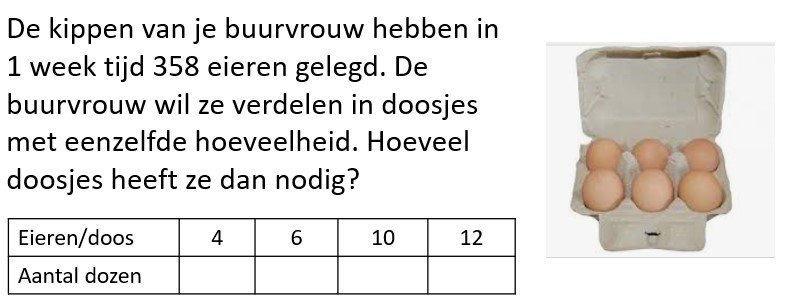
\includegraphics[width=\linewidth]{img/kippen.jpg} 

Het valt op dat de vraagontwerpers de leerlingen erg graag een verhoudingstabel willen voorschotelen. Alleen roept deze probleemstelling nog veel meer vragen op. Een buurvrouw wiens kippen in totaal 358 eieren leggen? Werkelijk? Een prachtige, authentieke vraag zou eerst en vooral zijn: hoeveel kippen heeft die buurvrouw dan? (Het antwoord: een snelle zoektocht op internet leert dat een gemiddelde kip ongeveer 5 eieren per week legt. Het gaat dus over een 72-tal kippen. We kunnen hier niet echt spreken over een doorsnee buurvrouw).

Tot slot hebben zeer veel functionele contexten met geld te maken. Het is zeker niet verkeerd dat als het over basisgeletterdheid gaat, de link naar rekenen met geld wordt gelegd. Toch is gecijferdheid rijker en is het raadzaam waakzaam te blijven dat niet alle vragen in het kader van bewerkingen met getallen, over geld gaan.


\section{Gecijferdheid evalueren}
Is het nodig om al deze doelen summatief te evalueren? Neen, afhankelijk de keuze voor een inductieve, dan wel deductieve aanpak, is een summatieve evaluatie op het niveau van de basisgeletterdheid raadzaam. 

Een volledige summatieve evaluatie is niet verplicht. Sommige scholen kiezen voor een periodieke toetsing van basisgeletterdheid, bv. aan de start van het eerste jaar, het einde van het eerste jaar en het einde van het tweede jaar. Nog andere scholen ontwikkelden een vragendatabank waaruit de leraar kan putten als er leerlingen voor sommige reguliere eindtermen dreigen uit te vallen of om na te gaan of ze het niveau de basisgeletterdheid bereiken. Een aanpak waarbij de vakgroep (digitale) toetsen heeft klaarliggen wanneer een leerling uitvalt op de reguliere toets waaraan enkele doelen basisgeletterdheid onderliggend zijn, is ook een handige aanpak.

Tijdens het masterproefonderzoek van studenten Enya Vermeyen en Britt Lenaerts van de educatieve master wiskunde aan de Universiteit Antwerpen, werden er in samenwerking met de professionele leergemeenschap wiskunde van het stedelijk- en gemeentelijk onderwijs (OVSG) valide toetsvragen ontwikkeld rond de doelen basisgeletterdheid getallenleer en de doelen meetkunde. 

Beide studenten ontwierpen bij de ontwikkeling van de toets een toetsmatrijs, die de vragen indeelde in drie niveaus: makkelijk, middelmatig, moeilijker. Het voordeel aan zo'n toetsmatrijs is dat het erg eenvoudig wordt om gelijkwaardige toetsen te ontwerpen. De ontwikkelde toetsmatrijzen, alsook de instaptoetsen vind je op onze website. Een stukje van een toetsmatrijs rond het interpreteren van tabellen, vind je in de onderstaande tabel. 

In het volgende stukje geven we enkele voorbeeldvragen uit het interpreteren van tabellen, getallenleer en meetkunde met telkens vragen van de verschillende niveaus.
\end{multicols}
\begin{tabel}
	\begin{tabular}{p{0.18\linewidth}p{0.24\linewidth}p{0.24\linewidth}p{0.24\linewidth}}
	\hlinethick
 \multicolumn{1}{c}{\tableheader{Doel}} & \multicolumn{1}{c}{\tableheader{Niveau 1 - Makkelijk}} & \multicolumn{1}{c}{\tableheader{Niveau 2 - Middelmatig}} & \multicolumn{1}{c}{\tableheader{Niveau 3 - Moeilijk}} \\
  \hlinethick
\textbf{De leerlingen interpreteren tabellen in functionele contexten.}   & Uit een gegeven tabel rechtstreeks informatie kunnen aflezen als antwoord op de vraag.  &  Uit een gegeven tabel informatie kunnen aflezen om een afweging te maken.   & Uit een gegeven tabel informatie kunnen aflezen en één bewerking uitvoeren om tot het antwoord op de vraag te komen.
\end{tabular}
	\caption{Voorbeeld van een rij uit een toetsmatrijs} \label{tab:matrijs}
\end{tabel}

\begin{multicols}{2}
\textbf{Interpreteren van tabellen}\\
  Jaarlijks publiceert Statbel de populairste voornamen van jongens en meisjes geboren in België. In \autoref{voornamen} vind je de top 5 van sterkste stijgers en dalers van meisjesnamen over de periode 2011-2021. Hieronder vind je voor elk niveau uit de toetsmatrijs een voorbeeldvraag. 
\afbeelding{img/voornamen.jpg}{Top 5 sterkste stijgers en dalers meisjesnamen 2011-2021}{voornamen}

\begin{vraagenantwoord}
		\vraag{\textbf{Makkelijk} - Hoeveel baby's kregen de voornaam Julie in België in 2021?}
		\antwoord{170 keer}
		\vraag{\textbf{Middelmatig} - Een koppel verwacht een meisje en twijfelt tussen `Ellis' en `Lotte' als naam. Ze willen vooral vermijden dat hun kindje steeds in klassen komt te zitten waar er ook andere leerlingen dezelfde naam hebben. Welk advies geef je hen op basis van deze tabel? Formuleer je advies in een zin.}
		\antwoord{Lotte komt 135 keer voor in 2021 als voornaam voor pasgeborenen, Ellis 125 keer. Beide voornamen waren in 2021 dus ongeveer even populair. Toch is Ellis op 10 jaar tijd veel populairder geworden. Als de baby in 2023 wordt geboren, heeft Ellis als voornaam Lotte waarschijnlijk ingehaald. Om het risico op twee Ellissen in de klas te vermijden, zou ik dus voor Lotte kiezen. }
		\vraag{\textbf{Moeilijk} - Wat is de procentuele afname van de voornaam  `Anaïs' op 10 jaar tijd? Rond af op één decimaal.}
		\antwoord{95/215= 44,2$\%$}
\end{vraagenantwoord}


\end{multicols}

\begin{lesactiviteit}{Basisgeletterdheid wiskunde met DuoLingo}
Duolingo is al jarenlang 's werelds populairste website en app om een andere taal te leren. De app dankt zijn populariteit onder meer door zijn speelse en intuïtieve benadering van het leerproces. Met wekelijkse toernooien en uitdagingen, die je samen met een vriend aangaat, probeert de app de motivatie hoog te houden. Ondertussen doe je de spraak- en luisteroefeningen en vertaal je zinnetjes, zodat je op je vakantieadres uit de voeten kunt. 

Sinds oktober 2022 heeft Duolingo ook een app om wiskunde te leren. De opdrachten starten met eenvoudige optelsommen, maar snel krijgen leerlingen te maken met breuken, decimalen, oppervlakte, omtrek en hoeken berekenen. Ook kloklezen en rekenen met tijd komen aan bod. 

De meeste wiskundeopdrachten hebben een vergelijkbare lay-out als de taallessen van Duolingo en rond je in enkele minuten af. De gewone opdrachten worden afgewisseld met uitdagingen en minigames. Elke oefening is anders. Hoewel de app voorlopig alleen maar in het Engels beschikbaar is, lijkt het een handige tool om leerlingen die het wat moeilijker hebben met gecijferdheid, alvast op weg te helpen. 
\afbeelding[6cm]{img/duolingo.jpg}{}{}
\end{lesactiviteit}

\begin{multicols}{2}
\textbf{Niveau 1: Elementair - Meetkunde}\\
\noindent Conceptuele kennis - Onderscheid tussen omtrek en oppervlakte\\

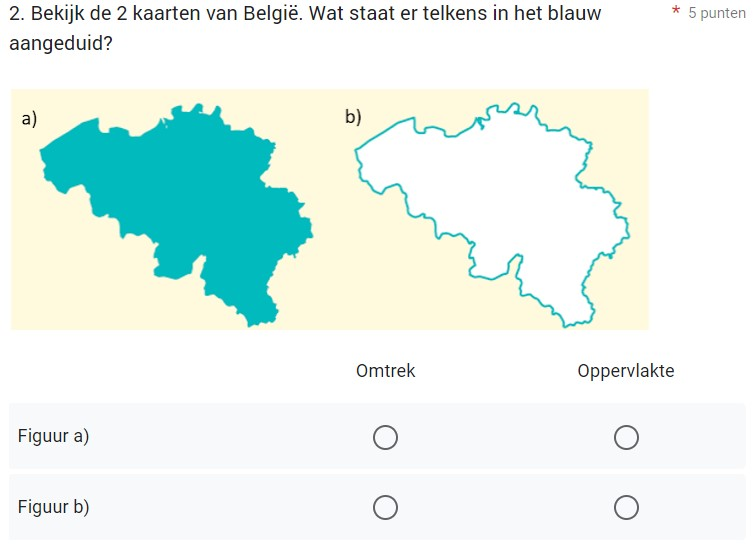
\includegraphics[width=\linewidth]{img/m1.jpg}


\textbf{Niveau 2: Gemiddeld - Meetkunde}\\
\noindent Meetkundige relaties in het vlak: loodrechte stand en evenwijdige rechten

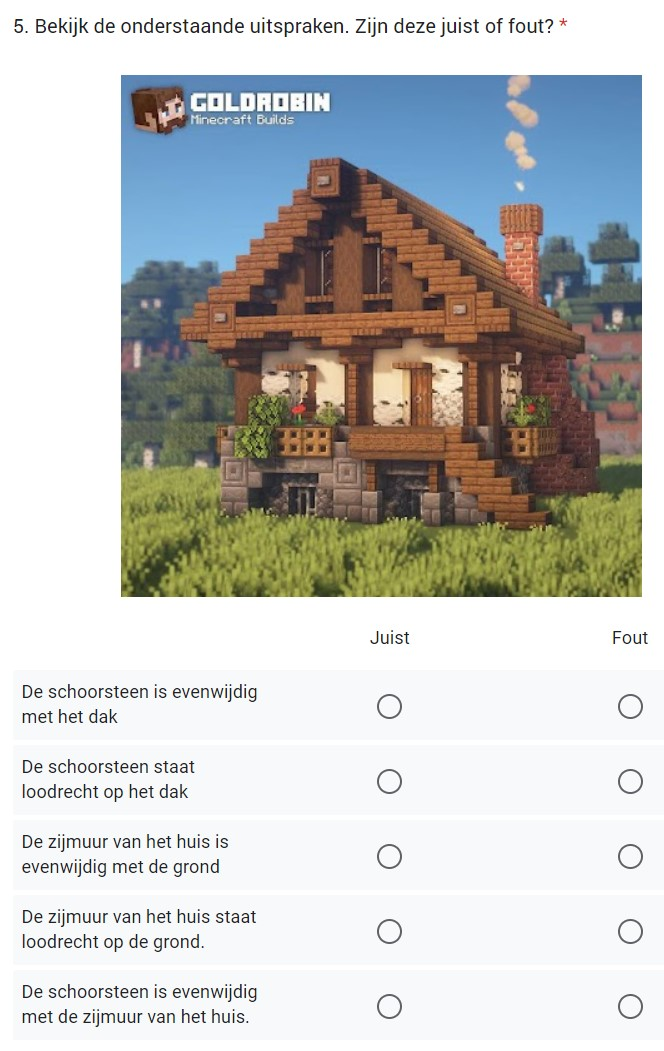
\includegraphics[width=\linewidth]{img/m2.jpg}

\textbf{Niveau 3: Moelijker - Meetkunde}\\
\noindent Meetkundige objecten herkennen (Driehoek, Vierhoek, Vierkant, Rechthoek, Cirkel, Balk, Kubus, Bol)

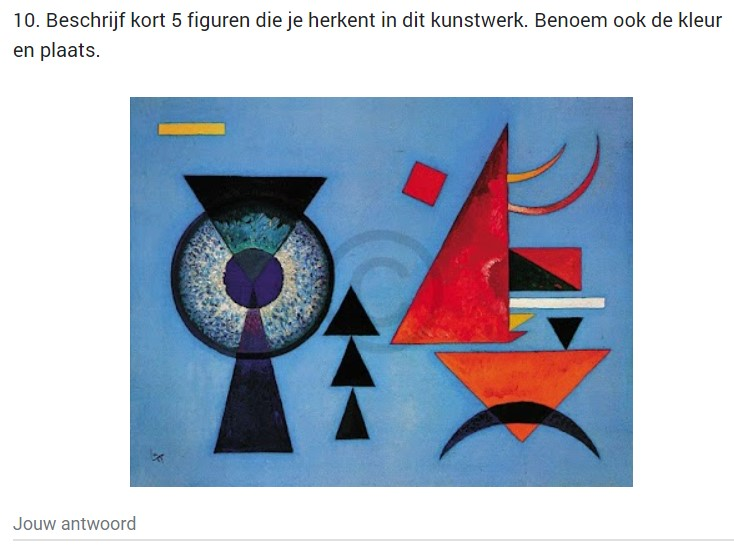
\includegraphics[width=\linewidth]{img/m3.jpg}

\textbf{Niveau 1: Elementair - Getallenleer}\\
\noindent Getallen, schatten, afronden - inschatten van de grootte-orde van een getal.

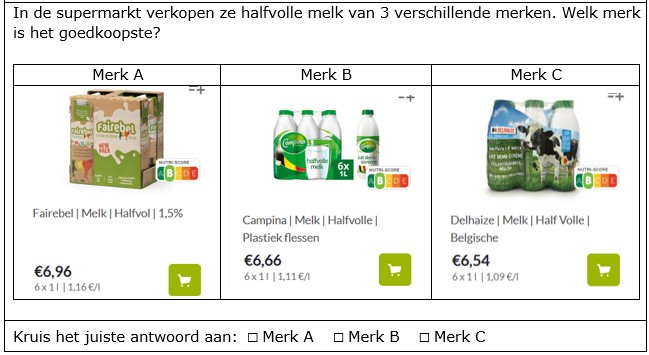
\includegraphics[width=\linewidth]{img/g1.jpg}

\textbf{Niveau 2: Gemiddeld - Getallenleer}\\
\noindent Hoofdbewerkingen - Delen en vermenigvuldigen.

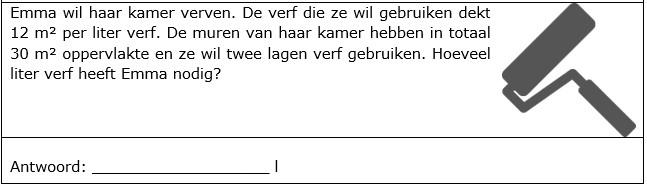
\includegraphics[width=\linewidth]{img/g2.jpg}

\textbf{Niveau 3: Moeilijker - Getallenleer}\\
\noindent Getallen, schatten, afronden - inschatten van de grootte-orde van een getal.

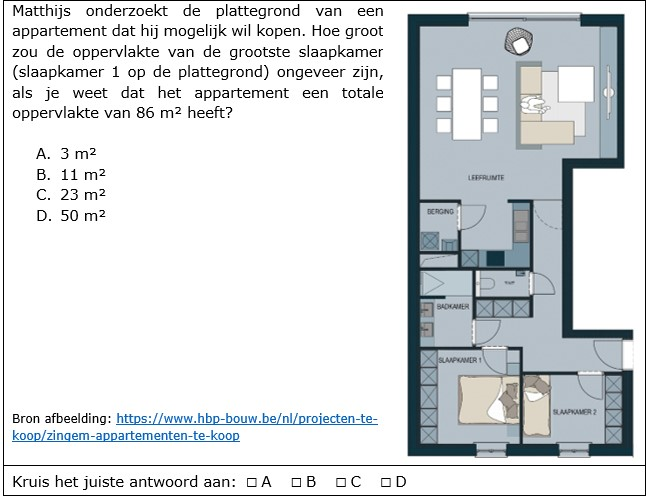
\includegraphics[width=\linewidth]{img/g3.jpg}


\section{Eerste wetenschappelijke bevindingen}
In de marge van de twee masterproeven van de studenten, werd er tijdens de validatie van de vragen van getallenleer bij 109 leerlingen aan Antwerpse stadsscholen van zowel 1A, 1B als 2A en 2B extra informatie vergaard om enkele aanvullende  onderzoeksvragen na te gaan: (1) Is focussen op de reguliere eindtermen genoeg om ook de basisgeletterdheid te bereiken? (2) Zijn rapportcijfers een goede voorspeller voor het halen van de basisgeletterdheid? (3) Hoe goed kunnen wiskundeleraars bij hun leerlingen het bereiken van de basisgeletterdheid inschatten? 

Bij het lezen van de resultaten en conclusies is het belangrijk om in het achterhoofd te houden dat het om een niet-representatieve steekproef gaat. Het betreft uitsluitend Antwerpse stadsscholen die allemaal nog niet gestart waren met de basisgeletterdheid.

Als we kijken naar het gemiddelde resultaat (score op 20) op de test rond getallenleer van de leerlingen, dan vallen er ons in \autoref{tab:deel} een aantal zaken op. Vooreerst zijn de resultaten verrassend laag, zeker gezien het erg elementaire niveau van de vragen. Zoals verwacht scoren de leerlingen uit 1B het minst, met gemiddeld 8,6/20, en de leerlingen uit 2A het meest met 13,1/20. Aanvankelijk verwachtten de onderzoekers veel hogere gemiddeldes, zeker voor de A-stroom.

\begin{tabel}
\centering
\begin{tabular}{llc}
	\hlinethick
\tableheader{\begin{tabular}[c]{@{}l@{}}Klas\end{tabular}} &
  \tableheader{\begin{tabular}[c]{@{}l@{}}Aantal\\ leerlingen\end{tabular}} &
  \tableheader{\begin{tabular}[c]{@{}l@{}}Gemiddelde score\\ $\pm$ St.dev\end{tabular}} \\
  	\hlinethick
1B & 25 & 8,6 $\pm$ 2,4  \\
2B & 25 & 10,6 $\pm$ 2,4 \\
1A & 23 & 12,7 $\pm$ 2,6 \\
2A & 36 & 13,1 $\pm$ 1,9
\end{tabular}

	\caption{Deelnemende klassen en resultaten test getallenleer} \label{tab:deel}
\end{tabel}

\textbf{Onderzoeksvraag 1: Is focussen op de reguliere eindtermen om de eindtermen basisgeletterdheid te halen?}\\

\noindent Het antwoord op deze vraag vinden we deels door na te gaan of de resultaten in \autoref{tab:deel} voldoende van elkaar verschillen. Wat blijkt? Alle groepen verschillen significant van elkaar - ook  1B en 2B ($p = 0,01$), op één vergelijking na: tussen 1A en 2A kunnen we op basis van de resultaten geen signficant onderscheid maken ($p=0,87$). Dit impliceert dat een extra jaar wiskundeonderwijs (zonder expliciete aandacht voor de basisgeletterdheid), in de A-stroom niet per se een verbetering van het beheersen van de basisgeletterdheid met zich meebrengt. 

Deze analyse lijkt te suggereren dat er in de B-stroom dichter rond de eindtermen basisgeletterdheid gewerkt wordt omdat ook de reguliere eindtermen van de B-stroom er meer op lijken. Dit rendeert naar beheersing van de eindterm  basisgeletterdheid, terwijl de beheersing van de eindterm getallenleer uit de basisgeletterdheid niet significant verbetert tussen het eerste en tweede jaar van de A-stroom.

In de A-stroom gaat men in de praktijk er vaak vanuit dat leerlingen die mee kunnen in de gewone lessen wiskunde van de A-stroom de eindtermen basisgeletterdheid wiskunde wel zullen beheersen op het einde van de eerste graad van het secundair onderwijs. Verder veronderstelt men meestal dat werken aan de eindtermen wiskunde voor de A-stroom ook helpt bij de beheersing van de eindtermen basisgeletterdheid wiskunde. Deze resultaten ontkrachten deels deze stelling, al blijft het een onderzoek op een niet-representatieve steekproef. 

\textbf{Onderzoeksvraag 2: Hoe voorspellen rapportcijfers de score op de test basisgeletterdheid getallenleer?}\\

Naast het afnemen van de test basisgeletterdheid wiskunde in mei 2022, vroegen we bij de deelnemers de rapportcijfers op voor de vakken wiskunde en Nederlands. Voor 1B en 2B zijn de rapportscores de punten voor het dagelijks werk en voor 1A en 2A zijn de rapportscores de punten bij de examens na het eerste trimester. De rapportscores werden telkens uitgedrukt in een percentage. Vervolgens werd de behaalde score op de test basisgeletterdheid getallenleer vergeleken met de rapportscore voor wiskunde en met de rapportscore voor Nederlands. Intuïtief zouden we verwachten dat de rapportcijfers voor wiskunde sterk correleren met het testresultaat op de basisgeletterdheid. De correlaties vindt u in \autoref{rapprotcijfers}. 
\end{multicols}

\begin{tabel}
\centering
\begin{tabular}{llll}
	\hlinethick
\tableheader{Klas} &
  \tableheader{\begin{tabular}[c]{@{}l@{}}Correlatie toetsscore \& \\rapportcijfer wiskunde\end{tabular}} &
  \tableheader{\begin{tabular}[c]{@{}l@{}}Correlatie toetsscore \& \\rapportcijfer Nederlands\end{tabular}} &
 \tableheader{ \begin{tabular}[c]{@{}l@{}}Correlatie rapportcijfers\\ wiskunde \& Nederlands\end{tabular}} \\
  	\hlinethick

1B & 0,18 & 0,24 & 0,43 \\
2B & 0,50 & 0,35 & 0,65 \\
1A & 0,41 & 0,39 & 0,75 \\
2A & 0,24 & 0,13 & 0,54
\end{tabular}
\caption{Correlaties tussen de toetsscores op de toets basisgeletterdheid getallenleer en de rapportcijfers voor wiskunde \& Nederlands} \label{rapprotcijfers}
\end{tabel}
\begin{multicols}{2}
Het valt op dat de meeste correlaties erg zwak zijn (< 0,5). Gewone rapportcijfers voor wiskunde lijken dus niet zo'n goede voorspeller voor het bereiken van de basisgeletterdheid, althans voor getallenleer. De rapportcijfers van de vakken Nederlands en wiskunde correleren veel sterker met elkaar dan met de score op de test basisgeletterdheid getallenleer. 

Een mogelijke verklaring is dat de ontwikkelde test volledig onvoorbereid werd afgenomen. Daardoor is dit een toets van parate kennis en transfervaardigheden tussen de klaspraktijk en een nieuwe situatie. Dit is helemaal iets anders dan toetsen dagelijks werk of een examen waar de leerling voor kan studeren. Bovendien is, zeker in 1B, nog niet alles van de basisgeletterdheid getallenleer reeds aan bod gekomen. Een lage correlatie was dus te verwachten. Toch is het antwoord op de onderzoeksvraag: nee, rapportcijfers zijn over het algemeen geen goede voorspellers voor het bereiken van de basisgeletterdheid wiskunde. Dit duidt ook op wat in deze loep al meermaals werd aangehaald: gecijferdheid is echt geen synoniem voor wiskunde.

\textbf{Onderzoeksvraag 3: Hoe goed kunnen wij als leraars wiskunde bij onze leerlingen voorspellen wie de basisgeletterdheid beheerst?}\\

We vroegen de leerkrachten wiskunde van 1B, 2B, 1A en 2A vooraf om voor elke leerling een prognose te maken over het al dan niet slagen op de test basisgeletterdheid getallenleer. Bij een positieve prognose verwachtte de leerkracht dat die leerling zou slagen op de test en bij een negatieve prognose verwachtte de leerkracht dat die leerling niet zou slagen.
\end{multicols}

\begin{tabel}
\centering
\begin{tabular}{lllll}
	\hlinethick
\tableheader{} &
\multicolumn{2}{l}{\tableheader{\begin{tabular}[c]{@{}l@{}}Positieve prognose door  leerkracht\end{tabular}}} &
\multicolumn{2}{l}{\tableheader{\begin{tabular}[c]{@{}l@{}}Negatieve prognose door leerkracht\end{tabular}}} \\
\tableheader{Klas}&
 \begin{tabular}[c]{@{}l@{}}Geslaagd  op de test\end{tabular} &
\begin{tabular}[c]{@{}l@{}}Niet geslaagd op de test\end{tabular} &
\begin{tabular}[c]{@{}l@{}}Geslaagd op de test\end{tabular}&
\begin{tabular}[c]{@{}l@{}}Niet geslaagd op de test\end{tabular} \\
  	\hlinethick
1B     & 7  & 11 & 1  & 6  \\
2B     & 13 & 6  & 5  & 1  \\
1A     & 9  & 0  & 9  & 5  \\
2A     & 28 & 1  & 6  & 1  \\
	\hlinethick
\textbf{Totaal} & \textbf{58} & \textbf{17} &\textbf{21} & \textbf{13}\\
	\hlinethick
\end{tabular}
\caption{Het aantal leerlingen dat geslaagd of juist niet geslaagd was op de instaptoets met een positieve prognose van de leerkracht of met een negatieve prognose van de leerkracht voor elke groep (1B, 2B, 1A en 2A) en voor de totale groep. In deze vergelijking werden leerlingen met een score van minstens 10/20 als geslaagd beschouwd.} \label{voorspellen}
\end{tabel}

\begin{multicols}{2}

In \autoref{voorspellen} vind je terug in hoeverre de prognose van de leerkracht overeenkwam met het echte behaalde resultaat op de test (geslaagd of niet geslaagd, waarbij we uitgaan van de gangbare cesuur van 10/20). Uit deze gegevens kan je aflezen dat de prognose van de leerkracht zeker een meerwaarde heeft. Van de leerlingen met een negatieve prognose was 38$\%$ niet geslaagd op de instaptoets, terwijl er van de leerlingen met een positieve prognose slechts 23$\%$ niet geslaagd was. 

Toch is dit verband niet significant: het aandeel geslaagden verschilt niet tussen leerlingen met een positieve of negatieve prognose door de leerkracht. De test kon bijgevolg nog meer leerlingen identificeren met problemen op vlak van basisgeletterdheid getallenleer dan men op basis van de prognose van de leerkrachten of de rapportpunten kon inschatten. Vermoedelijk kan dit verschil verklaard worden door het feit dat sommige leerlingen wel goed zijn in het studeren voor en presteren op toetsen, maar achteraf veel leerstof vergeten en het dan vervolgens slecht doen op een volledig onverwachte toets die peilt naar hun parate kennis. Daarnaast valt met dit onderzoeksresultaat opnieuw op dat gecijferdheid echt wat anders is dan het vak wiskunde zelf.

\section{Wat verwacht de inspectie?}
Wanneer de vakgroep discussieert over een zinvolle invulling van de doelen basisgeletterdheid bij jou op school, hou dan vooral je leerlingenpubliek in het achterhoofd. Dit bepaalt immers welke acties de vakgroep moet ondernemen om hen zo ver mogelijk te brengen in zowel de basisgeletterdheid als de reguliere doelen. De vraag `Wat gaat de inspectie daarvan vinden?' is daarbij niet de belangrijkste. Je geeft les voor je leerlingen, je moet uitsluitend voor hen de juiste beslissingen nemen. Bij een goede uitrol, zal de inspectie meegaan in jullie verhaal. 

De onderwijsinspectie formuleerde in hun `FAQ modernisering 1$^\text{e}$ graad so' in vraag-en-antwoord vorm een aantal verwachtingen ten aanzien van de basisgeletterdheid voor wiskunde. We nemen de relevante passages hier letterlijk over.

\begin{vraagenantwoord}
		\vraag{Volstaat het dat een leraar de `verwante' eindtermen basisvorming aanbiedt/evalueert en pas `teruggrijpt' naar de eindtermen basisgeletterdheid wanneer de leerling de eindtermen basisvorming niet behaalt?}
		\antwoord{Ja, dit volstaat, mits enige alertheid voor de basisgeletterdheid wiskunde, waarbij sommige doelen toch anders geformuleerd zijn dan de doelen voor wiskunde zelf (bv. het verschil tussen verhoudingen en breuken). Indien een leerling de ‘verwante’ eindterm van de basisvorming niet behaalt, gaat de school na of de leerling de eindtermen basisgeletterdheid behaalt. Daarbij respecteert de leraar de eigenheid van de eindtermen basisgeletterdheid:\begin{itemize}
    \item de eindtermen basisgeletterdheid kenmerken zich door hun realisatie in een functionele context,
    \item er is soms een verschil in het gevraagd beheersingsniveau en/of afbakening,
    \item de realisatie voor elke individuele leerling. 
\end{itemize}}
		
		\vraag{Kunnen we ervan uitgaan dat leerlingen in de A-stroom de eindtermen basisgeletterdheid
reeds behaald hebben in het basisonderwijs?}
		\antwoord{Neen, want (1) de eindtermen basisgeletterdheid zijn te behalen op individueel niveau (t.o.v. populatieniveau eindtermen basisonderwijs); (2) eindtermen basisgeletterdheid zijn te behalen op het einde van de eerste graad; (3) Eindtermen basisgeletterdheid zijn afgeleid van de eindtermen van de B-stroom.}
		
				\vraag{Moet een school de realisatie van de eindtermen basisgeletterdheid voor elke individuele leerling in kaart brengen?}
		\antwoord{Neen, maar leraren en scholen hebben wel een zicht op welke leerlingen mogelijk de eindtermen basisgeletterdheid niet behalen. Dit is een belangrijk gegeven voor de klassenraad, zowel de begeleidende als de delibererende. De begeleidende klassenraad heeft deze informatie nodig in functie van remediëring en differentiatie, de delibererende met het oog op attestering.}
		
    \vraag{Wat als een leerling de eindtermen basisgeletterdheid niet bereikt? Kan een leerling een A-attest behalen als hij één of meerdere eindtermen basisgeletterdheid niet behaald heeft?}
    \antwoord{Ja, want de delibererende klassenraad is het enige orgaan op het vlak van de beslissingen inzake het al dan niet geslaagd zijn.
De eindtermen basisgeletterdheid moeten door elke individuele leerling worden bereikt op het einde
van de eerste graad. Basisgeletterdheid zijn die eindtermen die ertoe strekken te kunnen
participeren in de maatschappij. In uitzonderlijke gevallen kan de klassenraad gemotiveerd beslissen
dat een individuele leerling een eindterm basisgeletterdheid niet moet bereiken.}
\vraag{Moet een school rapporteren over de realisatie van de eindtermen basisgeletterdheid?}
\antwoord{Ja, maar enkel wanneer een leerling een eindterm basisgeletterdheid niet behaalt. Dan verwachten
we in de notulen van de delibererende klassenraad op het einde van de eerste graad, bij een A- of B-attest een beknopte motivering waarom een individuele leerling alsnog slaagt.
Waar de realisatie van de eindtermen van de basisvorming of van de eindtermen basisgeletterdheid
in het gedrang komt, verwachten we daarover een transparante en tijdige communicatie naar de leerling en de ouders.}
	\end{vraagenantwoord}
\end{multicols}


\newpage

\begin{lesactiviteit}{Taalsteun voor taalzwakke leerlingen}
\textbf{\textit{Bron: Manon Froklage \& Gwendolien Depré, Taalontwikkeld wiskundelesgeven in de B-stroom, B+ project}}

Uit tal van wetenschappelijk onderzoek (Prediger \& Wessel, 2013) weten we dat er een innige band is tussen de beheersing van taal en wiskunde: een leerling die goed scoort op taal, scoort gemiddeld genomen ook beter voor wiskunde. Voor sommige leerlingen zijn dan ook de wiskundige bewerkingen niet het grootste probleem, maar de taal waarin sommige vraagstukken wordt verpakt. Hoewel de band tussen taal en wiskunde al uitgebreid is besproken in de loep `Wiskunde en taal' van Uitwiskeling 29/2, geven we enkele tips om taalontwikkelend les te geven.

\textbf{Hang woordenposters in de klas}\\
\noindent `In verhouding', het verschil tussen omtrek/oppervlakte... het vak wiskunde zit vol begrippen die voor sommige leerlingen, zeker in de B-stroom, niet evident zijn. Een manier om hiermee om te gaan is hen te ondersteunen met woordenposters die uitleg geven over courante begrippen. Hieronder een collage met enkele voorbeelden. \\
\afbeelding[12cm]{img/woordposter.png}{}{}

\textbf{Tekening walkie-talkie}\\
\noindent In deze oefening zitten leerlingen per twee tegenover elkaar. De ene leerling heeft een figuur vast, de andere kleurpotloden. De leerling met de figuur moet zo duidelijk mogelijk omschrijven wat hij op het kaartje ziet, zodat de andere leerling, zonder het kaartje te zien, een zo accuraat mogelijke tekening kan maken. Beide leerlingen hebben wiskundige woordenschat nodig om deze opdracht tot een goed einde te brengen.\\
\afbeelding[6.5cm]{img/mamoet.png}{}{}


\textbf{Invloed van taal}\\
Veel vragen in functionele contexten kunnen omgezet worden naar een vraag met afbeeldingen. Dat maakt ze doorgaans veel eenvoudiger voor leerlingen en vaak ook functioneler. Zie bijvoorbeeld het onderstaande voorbeeld (bron: Hoogland \& Stelwagen, 2022):

\afbeelding[6.5cm]{img/voorbeeldtaal.jpg}{}{}



Het enige gevaar is dat de vraag te simpel wordt en de informatie op een manier die niet realistisch is, wordt aangeboden. De onderstaande opgave is daarvan een mooi voorbeeld. Dezelfde vraag wordt zonder en met visuele ondersteuning gesteld. De verschijningsvorm met afbeeldingen is veel eenvoudiger dan de eerste opgave. Toch is het niet erg realistisch om de lengte en de breedte rechtstreeks op een badkamerraam af te lezen. Voor het werken rond de basisgeletterdheid, is een goede vuistregel om de informatie nodig voor een probleemstelling, zoveel mogelijk aan te bieden zoals dat in de echte wereld gebeurt.
\begin{center}
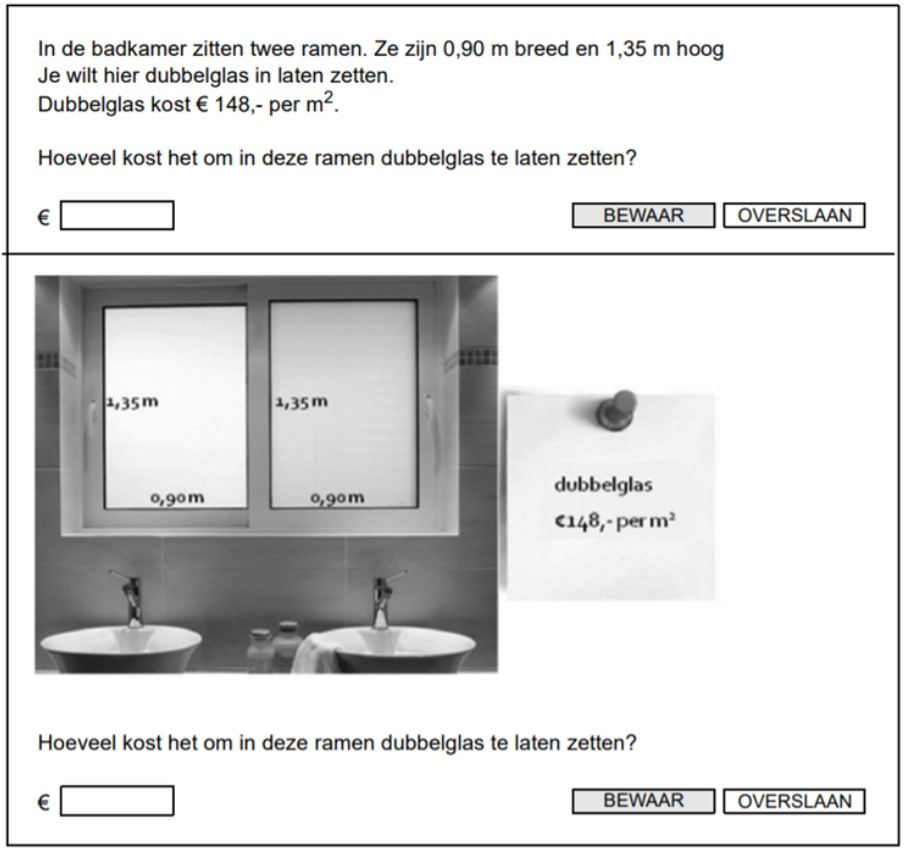
\includegraphics[width=0.6\linewidth]{img/effectvantaal.jpg}
\end{center}
\end{lesactiviteit}


	






\stopcontents[inhoudloep]		% om inhoud voor het loep artikel te eindigen


%% BRONNEN %%%%%%%%%%%%%%%%%%%%%%%%%%%%%%%%%%%%%%%%%%%%%%%%%%%%%%%%%%%%%%%%%%%%%
\begin{bronnen}
\item Balk, G.L., van Dijk, Frans, Kortlang, D.J. (2007). The archives of the Dutch East India Company (VOC) and the local institutions in Batavia (Jakarta), p. 46
\item Bregman, R. (2013). Waarom arme mensen domme dingen doen. \emph{De Correspondent}.
\item Hoogland, K., Stelwagen, R. (2022). Het belang van rekenen en gecijferdheid in een leven lang ontwikkelen. Hogeschool Utrecht. Geraardpleegd via \url{https://www.gecijferdheid.nl/category/publicaties/}.
\item Kemme, S., Wijers, M., Joncker, V. (2003). Authentieke contexten in wiskundemethoden in het VMBO. Geraadpleegd van \url{https://core.ac.uk/download/pdf/39704851.pdf}
\item Moons, F. (2021). Basisgeletterdheid Wiskunde: een didactische aanpak zonder planlast. Presentatie op de Inspiratiedag wiskunde in de eerste graad B-stroom georganiseerd door de Vlaamse Overheid. Presentatie: https://prezi.com/view/ZH9JTaEgPyzfS9yMqxJS/. Opname: https://youtu.be/iYkGLrv6Cf4.
\item Onderwijsinspectie Vlaamse Overheid (2022). FAQ modernisering 1$^\text{e}$ graad so. Geraadpleegd via \url{https://www.onderwijsinspectie.be/sites/default/files/atoms/files/FAQ_modernisering.pdf}.
\item Oonk, W., van Zanten, M., Keijzer, R. (2007). Gecijferdheid, vier eeuwen ontwikkeling. \emph{Panama-post} 26/3, 3-18.
\item Paulos, J. A. (1988). \emph{Innumeracy, mathematical illiteracy and its consequences}. Hill \& Wang
\item Prediger, S., Wessel, L. (2013).Fostering German-language learners’ constructions of meanings for fractions—design and effects of a language- and mathematics-integrated intervention. \emph{Math Ed Res J} 25, 435–456 https://doi.org/10.1007/s13394-013-0079-2
\item PISA 2018. Universiteit Gent, vakgroep Onderwijskunde.
\item Sap, S., Tuttens, M. (2019). Basisgeletterdheid in de eerste graad van het secundair onderwijs. Welke gevolgen zullen de eindtermen basisgeletterdheid met zich meebrengen? (Bachelorscriptie). Geraadpleegd van \url{https://www.scriptieprijs.be/sites/default/files/thesis/2019-09/Basisgeletterdheid%20in%20de%201e%20graad.pdf}

 

\end{bronnen}